Este capítulo presenta el seguimiento y control del proyecto, abordando la gestión del alcance, la evaluación de riesgos y el control temporal de las actividades desarrolladas.

\section{Gestión del alcance}
Durante el desarrollo del proyecto, el alcance se ha ido modificando mediante la supresión de algunas tareas y la incorporación de otras nuevas. Todas estas modificaciones fueron resultado del seguimiento y control bisemaneal realizado con los tres directores del proyecto. A continuación se presenta un resumen de las modificaciones realizadas:

\begin{itemize}
\item\textbf{Limitación de mejoras incorporadas: }el alcance inicial contemplaba dos mejoras técnicas que fueron reducidas por limitaciones de recursos. Primero, la implementación de un sistema RAG avanzado con recuperadores densos especializados y su correspondiente evaluación, lo cual requería una cantidad considerable de datos cuya captura habría demandado gran parte de la dedicación. En su lugar, se implementaron mecanismos RAG más sencillos, incorporando un sistema de recuperación híbrida en el módulo de memoria. Segundo, el ajuste de un modelo de lenguaje para la selección de herramientas, que fue sustituido por el entrenamiento de un modelo clasificador más simple debido a la dedicación horaria restante al final del proyecto.

Dichas reducciones del alcance se seleccionaron estratégicamente de forma que no influyesen sobre los objetivos del proyecto. Como se ha mencionado en capítulos previos, el alcance inicial era ambigüo y eran previsibles dichos cambios.
\item\textbf{Modificación de arquitecturas de interacción alternativas: }Inicialmente se había planteado una interacción directa entre los egentes especialistas como posible mejora. Esta idea se cambió por una exploración más profunda de las arquitecturas de orquestación, ya que se observó que incluir cadenas de agentes excesivas puede derivar en una degradación progresiva de la información.
\item\textbf{Sistema de citación: }la implementación de un sistema de citación no estaba contemplada en el alcance inicial del proyecto. Esta funcionalidad fue incorporada posteriormente durante el proceso de seguimiento con los directores, al identificarse como una mejora para permitir al usuario conocer las fuentes de información utilizadas por los agentes en sus respuestas.
\end{itemize}

\section{Gestión de riesgos}
En este apartado se enumeran los riesgos que se materializaron en incidencias durante el desarrollo del proyecto, detallando su impacto y las medidas correctivas implementadas.

\subsection{R1-Concurrencia exploratoria}
Este riesgo se materializó al encontrar la publicación ``Onboarding Buddy'', el cual proponía un enfoque muy parecido para la creación de un sistema de agentes con una fase de planificación dinámica. 

El impacto de este riesgo supuso más bien un beneficio, al surgir en la fase inicial del proyecto. Se analizó la implementación de dicho trabajo y se incorporó un enfoque similar en el agente planificador. 

\subsection{R2-Variabilidad del alcance}
Este riesgo se materializó al inicio del proyecto, en la fase de planificación y captura de requisitos. El desarrollo de dicha captura requirió de un mayor esfuerzo de lo previsto, ya que definir el alcance del proyecto fue más desafiante de lo esperado. 

Al alargarse esta fase, se decidió recortar la fase de la mejoras propuestas, para evitar que el proyecto se alargara más de lo previsto o que conllevase un sobrecoste horario significativo.

\subsection{R4-Filtrado de credenciales}
Este riesgo se materializó al accidentalmente incluir la clave de acceso al modelo de openAI en el repositorio del proyecto. El impacto de este riesgo fue nulo gracias a la segunda capa de seguridad implementada, que consistía en mantener el repositorio privado. Como medida, se anuló la clave de acceso y se creó una nueva por si en un futuro el repositorio se hiciera público.

\subsection{R5-Pérdida de recursos}
Este riesgo se materializó al inicio del proyecto, cuando por un error humano fue necesario formatear el equipo de desarrollo sin previo respaldo. El impacto fue mínimo por las copias de seguridad periódicas.

\section{Gestión del tiempo}
El proyecto sufrió una desviación al principio del proyecto, ya que la definición del alcance y requisitos del sistema llevó más tiempo del anticipado.
\subsection{Gestión de fechas}
La desviación mencionada supuso un retraso de aproximadamente dos semanas al inicio del proyecto respecto a la planificación inicial con todas las posibles mejoras por implementar. La Tabla \ref{tab:hitos_real} muestra los cronogramas de hitos del proyecto reales, destacando el fin tardío de la primera iteración. Este retraso se redujo a 10 días al fin de la iteración 4. El fin de la última iteración concordó con su planificación inicial. En esta última iteración habría sido posible la implementación de mejoras adicionales, pero debido a que los objetivos del proyecto habían sido logrados, y la dedicación horaria técnica había sido agotada, se decidió centrar los esfuerzos en la redacción de la presente memoria. 

\begin{table}[H]\centering
\begin{tabular}{|l|c|c|}
\hline
\multicolumn{1}{|c|}{\textbf{Hito}} & \multicolumn{1}{c|}{\textbf{Fecha estimada}} & \multicolumn{1}{c|}{\textbf{Fecha real}} \\
\hline
Inicio del proyecto & 25/02/2025 & 25/02/2025 \\
\hline
Fin Iteración 1 & 20/03/2025 & 2/04/2025 \\
\hline
Fin Iteración 2 & 01/04/2025 & 15/04/2025 \\
\hline
Fin Iteración 3 & 15/04/2025 & 29/04/2025 \\
\hline
Fin Iteración 4 & 29/04/2025 & 09/05/2025 \\
\hline
Fin Iteración 5 & 27/05/2025 & 30/05/2025 \\
\hline
Fin memoria & 14/06/2025 & Por determinar \\
\hline
Defensa del proyecto & Por determinar & Por determinar \\
\hline
\end{tabular}
\caption{Cronograma de Hitos del Proyecto}
\label{tab:hitos_real}
\end{table}

\subsection{Dedicaciones}
La Figura \ref{fig:horas_real} ilustra la tabla de dedicación horaria por tareas actualizada con los valores reales. Destacan dos sobrecostes horarios: el correspondiente a la primera iteración y el correspondiente a la cuarta iteración. Dichos sobrecostes implicaron la reducción del alcance, lo que redujo la dedicación en la quinta iteración, equilibrando la balanza. El sobrecoste final se puede atribuir a una dedicación superior de lo estimada a la redacción de la memoria, la cual resultó ser significativamente más costosa de lo esperado. 

\begin{figure}[h]
\centering
\adjustbox{center=\textwidth}{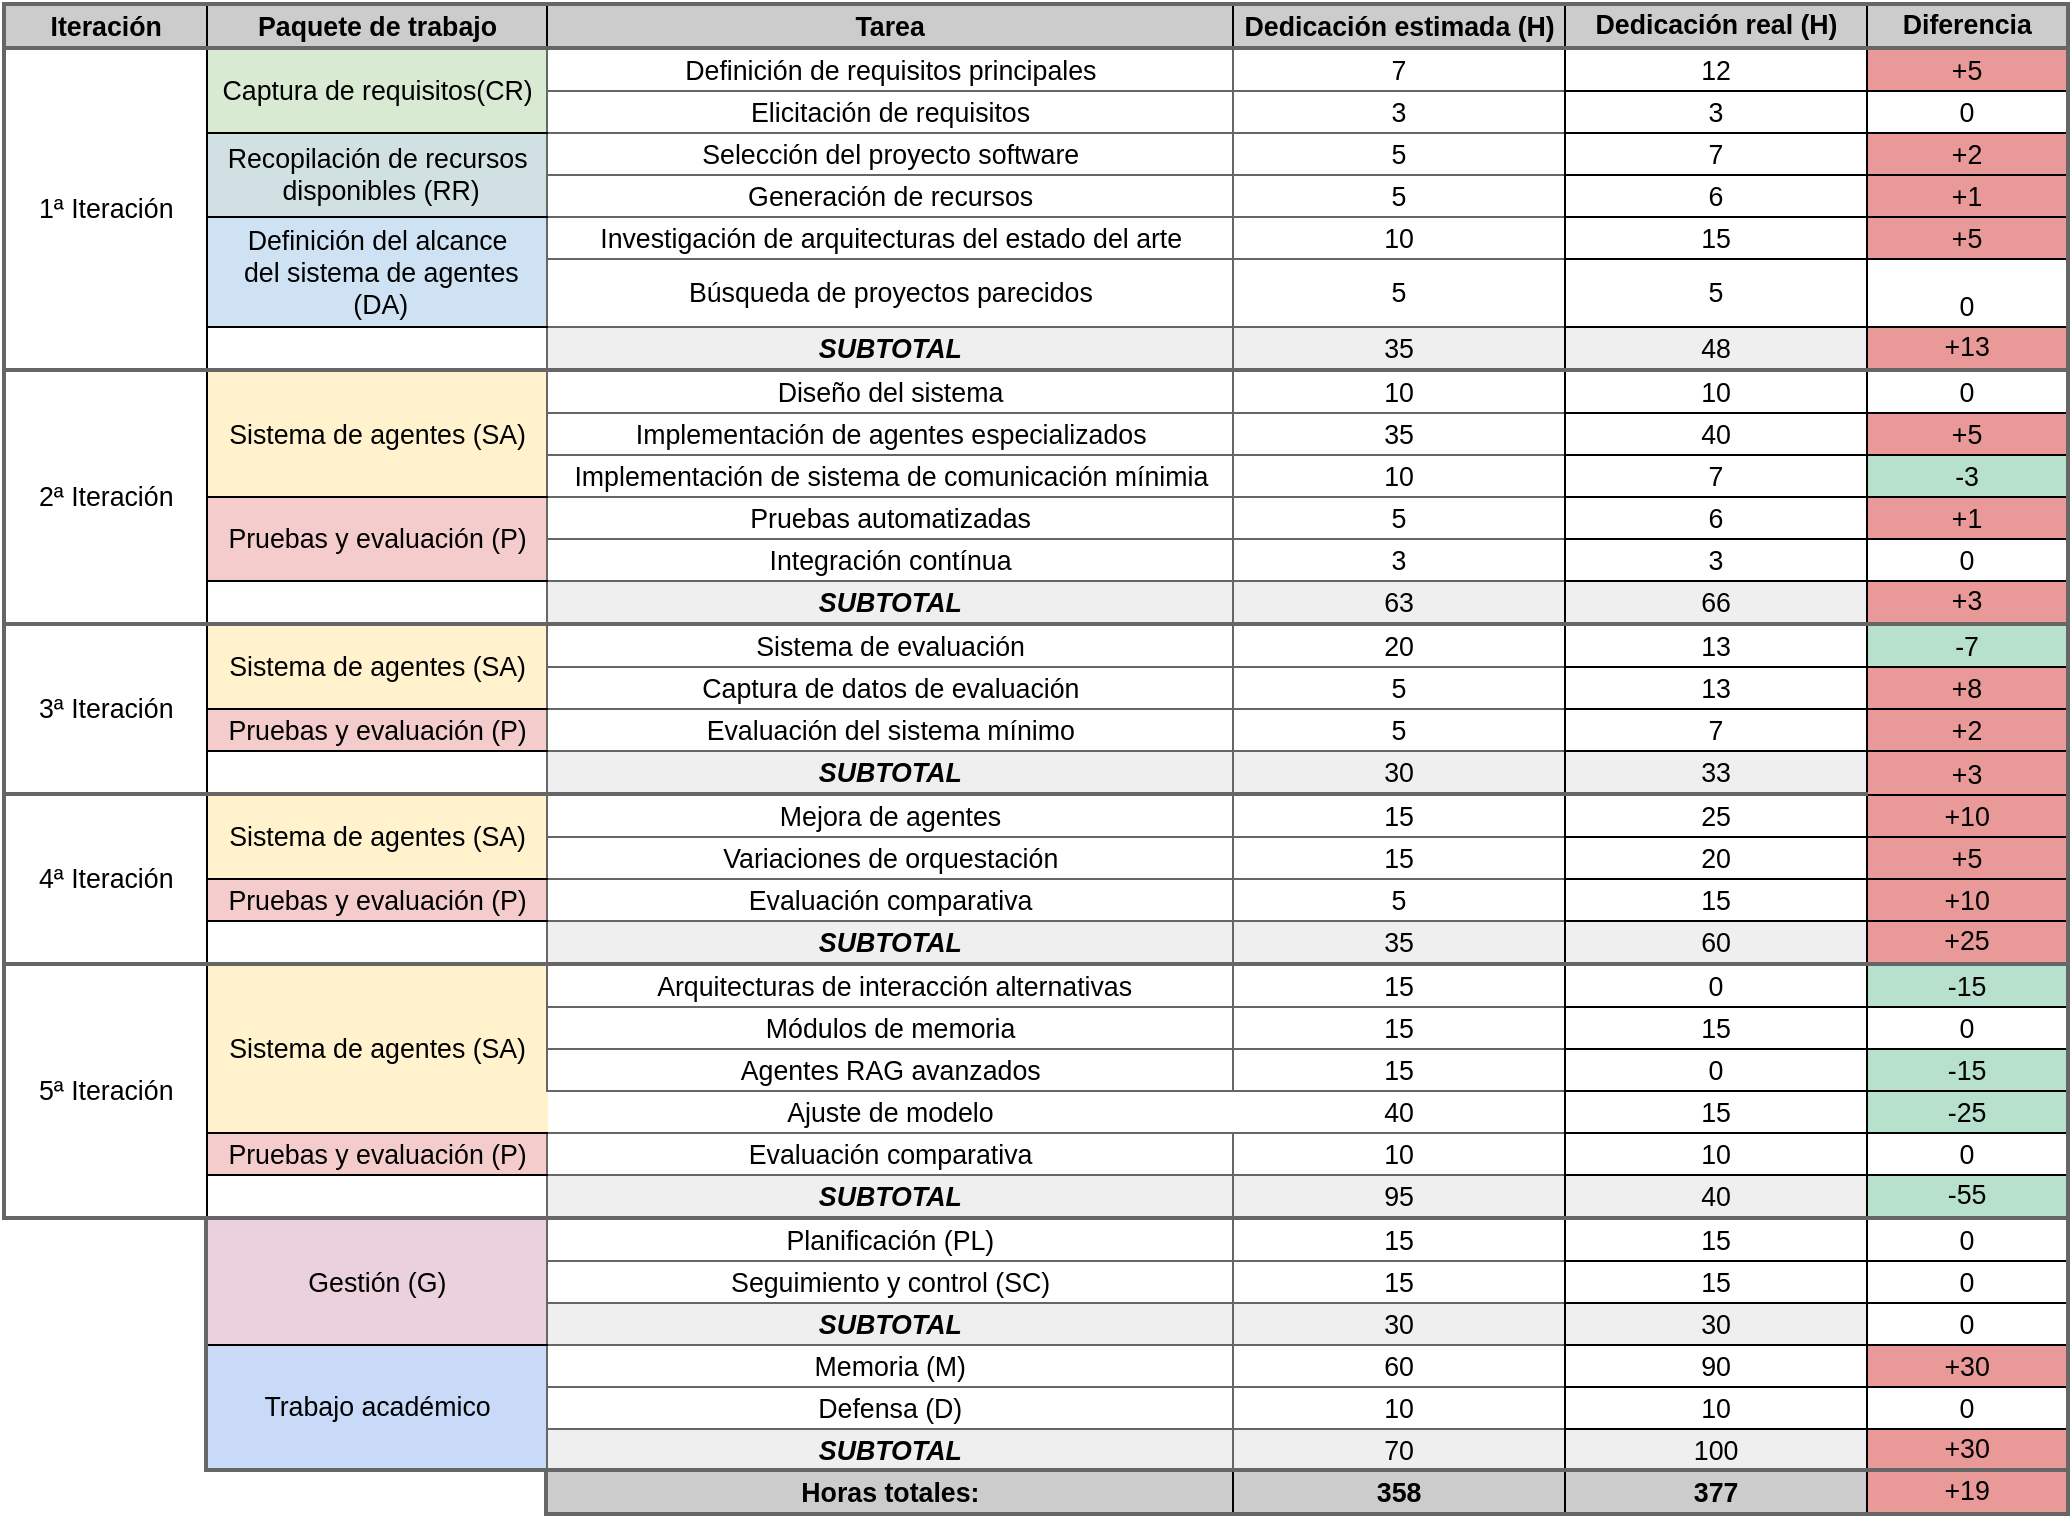
\includegraphics[width=1.3\linewidth]{figures/horas_real.png}}
\caption{Comparación de dedicación horaria estimada y real}
\label{fig:horas_real}
\end{figure}

El sobrecoste en la primera iteración se debe principalmente a la complicación a la hora de definir el alcance del sistema, lo cual implicó un 13 horas o un 37\% adicional. 

La segunda y tercera iteración fueron en general como lo planeado. Es de destacar que la implementación del sistema de evaluación fue más sencillo de lo previsto, con 7 horas o un 35\% menor de decicación. En cambio, pero la captura de los datos de evaluación fue más complejo de lo esperado, suponeindo un sobrecoste de 8 horas, o un 160\% de la tarea original.

La cuarta iteración fue también más compleja de lo esperado (+25 horas, +71\%), ya que se requirieron más correcciones del comportamiento inicial de lo esperado, necesitando 10 adicionales (60\%). La evaluación del sistema sufrió un sobrecoste significativo, de 10 horas o el 200\% de lo estimado. Esto se debe a que aunque la evaluación estaba automatizada, fue necesario el análisis de las ejecuciones en dicha evaluación para determinar los puntos débiles a mejorar.

Finalmente, la dedicación a la última iteración fue de aproximadamente la mitad de los esperado, debido a la reducción del alcance.

El sobrecoste de la memoria ha sido de 30 horas o del 50\%. Este se consideró razonable para la redacción de un documento digno. 

El sobrecoste total ascendió a 19 horas, equivalente al 5\% del proyecto. 






